%%%% Dokumentklassen %%%%

\documentclass[a4paper,11pt,fleqn,dvipsnames,twoside,openright]{memoir} 	% Openright åbner kapitler på højresider (openany begge)


%%%% PACKAGES %%%%

%% Oversættelse og tegnsætning %%
\usepackage[utf8]{inputenc}					% Input-indkodning af tegnsæt (UTF8)
\usepackage[danish]{babel}					% Dokumentets sprog
\usepackage[T1]{fontenc}					    % Output-indkodning af tegnsæt (T1)
\usepackage{ragged2e,anyfontsize}			% Justering af elementer
\usepackage{fixltx2e}						% Retter forskellige fejl i LaTeX-kernen

\usepackage{lastpage}						% Total antal sider opdateres automatisk ved \pageref{LastPage}
																			
%% Figurer og tabeller (floats) %%
\usepackage{graphicx} 						% Håndtering af eksterne billeder (JPG, PNG, EPS, PDF)
\usepackage{multicol}         	            	% Muliggør output i spalter
\usepackage{rotating}						% Rotation af tekst med \begin{sideways}...\end{sideways}
\usepackage{xcolor}							% Definer farver med \definecolor. Se mere: http://en.wikibooks.org/wiki/LaTeX/Colors
\usepackage{flafter}						% Sørger for at floats ikke optræder i teksten før deres reference
\let\newfloat\relax 						% Justering mellem float-pakken og memoir
\usepackage{float}							% Muliggør eksakt placering af floats, f.eks. \begin{figure}[H]

%% Matematik mm. %%
\usepackage{amsmath,amssymb,stmaryrd} 		% Avancerede matematik-udvidelser
\usepackage{mathtools}						% Andre matematik- og tegnudvidelser
\usepackage{textcomp}                 		% Symbol-udvidelser (fx promille-tegn med \textperthousand)
\usepackage{rsphrase}						% Kemi-pakke til RS-saetninger, fx \rsphrase{R1}
\usepackage[version=3]{mhchem} 				% Kemi-pakke til flot og let notation af formler, f.eks. \ce{Fe2O3}
\usepackage{siunitx}						% Flot og konsistent præsentation af tal og enheder med \si{enhed} og \SI{tal}{enhed}
\sisetup{output-decimal-marker = {,}}		% Opsætning af \SI (DE for komma som decimalseparator) 

%% Referencer og kilder %%
\usepackage[danish]{varioref}				% Muliggør bl.a. krydshenvisninger med sidetal (\vref)
\usepackage{natbib}							% Udvidelse med naturvidenskabelige citationsmodeller
\usepackage{xr}							    % Referencer til eksternt dokument med \externaldocument{<NAVN>}

%% Misc. %%
\usepackage{listings}						% Placer kildekode i dokumentet med \begin{lstlisting}...\end{lstlisting}
\usepackage{lipsum}							% Dummy text \lipsum[..]
\usepackage[shortlabels]{enumitem}			% Muliggør enkelt konfiguration af lister
\usepackage{pdfpages}						% Gør det muligt at inkludere pdf-dokumenter med kommandoen \includepdf[pages={x-y}]{fil.pdf}	
\pdfoptionpdfminorversion=6					% Muliggør inkludering af pdf-dokumenter, af version 1.6 og højere
\pretolerance=2500 							% Justering af afstand mellem ord (højt tal, mindre orddeling og mere luft mellem ord)


%%%% CUSTOM SETTINGS %%%%

%% Marginer %%
\setlrmarginsandblock{3.5cm}{2.5cm}{*}		% \setlrmarginsandblock{Indbinding}{Kant}{Ratio}
\setulmarginsandblock{2.5cm}{3.0cm}{*}		% \setulmarginsandblock{Top}{Bund}{Ratio}
\checkandfixthelayout 						% Oversætter værdier til brug for andre pakker

%% Afsnitsformatering %%
\setlength{\parindent}{0mm}           		% Størrelse af indryk
\setlength{\parskip}{3mm}          			% Afstand mellem afsnit ved brug af double Enter
\linespread{1,1}							% Linjeafstand

%% Indholdsfortegnelse %%
\setsecnumdepth{subsection}		 			% Dybden af nummererede overskrifter (part/chapter/section/subsection)
\maxsecnumdepth{subsection}					% Dokumentklassens grænse for nummereringsdybde
\settocdepth{subsection} 					% Dybden af indholdsfortegnelsen
		
%% Opsætning af listings %%
\definecolor{commentGreen}{RGB}{34,139,24}
\definecolor{stringPurple}{RGB}{208,76,239}

\lstset{language=Matlab,					    % Sprog
	basicstyle=\ttfamily\scriptsize,		    % Opsætning af teksten
	keywords={for,if,while,else,elseif,		% Nøgleord at fremhæve
			  end,break,return,case,
			  switch,function},
	keywordstyle=\color{blue},				% Opsætning af nøgleord
	commentstyle=\color{commentGreen},		% Opsætning af kommentarer
	stringstyle=\color{stringPurple},		% Opsætning af strenge
	showstringspaces=false,					% Mellemrum i strenge enten vist eller blanke
	numbers=left, numberstyle=\tiny,		    % Linjenumre
	extendedchars=true, 					    % Tillader specielle karakterer
	columns=flexible,						% Kolonnejustering
	breaklines, breakatwhitespace=true,		% Bryd lange linjer
}

%% Navngivning %%
\addto\captionsdanish{
	\renewcommand\appendixname{Appendiks}
	\renewcommand\contentsname{Indholdsfortegnelse}	
	\renewcommand\appendixpagename{Appendiks}
	\renewcommand\appendixtocname{Appendiks}
	\renewcommand\cftchaptername{\chaptername~}		% Skriver "Kapitel" foran kapitlerne i indholdsfortegnelsen
	\renewcommand\cftappendixname{\appendixname~}	% Skriver "Appendiks" foran appendiks i indholdsfortegnelsen
}

%% Kapiteludssende %%
\definecolor{numbercolor}{gray}{0.7}		            % Definerer en farve til brug til kapiteludseende
\newif\ifchapternonum

\makechapterstyle{jenor}{					        % Definerer kapiteludseende frem til ...
  \renewcommand\beforechapskip{0pt}
  \renewcommand\printchaptername{}
  \renewcommand\printchapternum{}
  \renewcommand\printchapternonum{\chapternonumtrue}
  \renewcommand\chaptitlefont{\fontfamily{pbk}\fontseries{db}\fontshape{n}\fontsize{25}{35}\selectfont\raggedleft}
  \renewcommand\chapnumfont{\fontfamily{pbk}\fontseries{m}\fontshape{n}\fontsize{1in}{0in}\selectfont\color{numbercolor}}
  \renewcommand\printchaptertitle[1]{%
    \noindent
    \ifchapternonum
    \begin{tabularx}{\textwidth}{X}
    {\let\\\newline\chaptitlefont ##1\par} 
    \end{tabularx}
    \par\vskip-2.5mm\hrule
    \else
    \begin{tabularx}{\textwidth}{Xl}
    {\parbox[b]{\linewidth}{\chaptitlefont ##1}} & \raisebox{-15pt}{\chapnumfont \thechapter}
    \end{tabularx}
    \par\vskip2mm\hrule
    \fi
  }
}											        % ... her

\chapterstyle{jenor}						        % Valg af kapiteludseende - Google 'memoir chapter styles' for alternativer

%% Sidehoved %%

\makepagestyle{AAU}							        % Definerer sidehoved og sidefod udseende frem til ...
\makepsmarks{AAU}{%
	\createmark{chapter}{left}{shownumber}{}{. \ }
	\createmark{section}{right}{shownumber}{}{. \ }
	\createplainmark{toc}{both}{\contentsname}
	\createplainmark{lof}{both}{\listfigurename}
	\createplainmark{lot}{both}{\listtablename}
	\createplainmark{bib}{both}{\bibname}
	\createplainmark{index}{both}{\indexname}
	\createplainmark{glossary}{both}{\glossaryname}
}
\nouppercaseheads									% Ingen Caps ønskes

\makeevenhead{AAU}{\small ST3PRJ3 Gruppe 4}{}{\leftmark}	% Definerer lige siders sidehoved (\makeevenhead{Navn}{Venstre}{Center}{Hoejre})
\makeoddhead{AAU}{\rightmark}{}{\small ASE}		            % Definerer ulige siders sidehoved (\makeoddhead{Navn}{Venstre}{Center}{Højre})
\makeevenfoot{AAU}{\small \thepage}{}{}						% Definerer lige siders sidefod (\makeevenfoot{Navn}{Venstre}{Center}{Højre})
\makeoddfoot{AAU}{}{}{\small \thepage}						% Definerer ulige siders sidefod (\makeoddfoot{Navn}{Venstre}{Center}{Højre})

\copypagestyle{AAUchap}{AAU}							% Sidehoved for kapitelsider defineres som standardsider, men med blank sidehoved
\makeoddhead{AAUchap}{}{}{}
\makeevenhead{AAUchap}{}{}{}
\makeheadrule{AAUchap}{\textwidth}{0pt}
\aliaspagestyle{chapter}{AAUchap}					% Den ny style vælges til at gælde for chapters
													% ... her
															
\pagestyle{AAU}										% Valg af sidehoved og sidefod


%%%% CUSTOM COMMANDS %%%%

%% Billede hack %%
\newcommand{\figur}[4]{
		\begin{figure}[H] \centering
			\includegraphics[width=#1\textwidth]{billeder/#2}
			\caption{#3}\label{#4}
		\end{figure} 
}

%% Specielle tegn %%
\newcommand{\decC}{^{\circ}\text{C}}
\newcommand{\dec}{^{\circ}}
\newcommand{\m}{\cdot}


%%%% ORDDELING %%%%

\hyphenation{}


%%%% Tilføjelser af min preample %%%%

% Booktabs:
% The booktabs package is needed for better looking tables. 
\usepackage{booktabs}

% Caption:
% For better looking captions. See caption documentation on how to change the format of the captions.
\usepackage[hang, font={small, it}]{caption}

% Hyperref:
% This package makes all references within your document clickable. By default, these references will become boxed and colored. This is turned back to normal with the \hypersetup command below.
\usepackage{hyperref}
	\hypersetup{colorlinks=false,pdfborder=0 0 0}

% Cleveref:
% This package automatically detects the type of reference (equation, table, etc.) when the \cref{} command is used. It then adds a word in front of the reference, i.e. Fig. in front of a reference to a figure. With the \crefname{}{}{} command, these words may be changed.
\usepackage{cleveref}
	\crefname{equation}{formel}{formler}
	\crefname{figure}{figur}{figurer}	
	\crefname{table}{tabel}{tabeller}

% Mine tilføjelser:
\usepackage{units}                        %% Bruges til at gøre fx 1/2 samlet med: \nicefrac{1}{2}.
\usepackage{tabu, longtable}              %% Bruges til tabeller.
\setlength{\tabulinesep}{1.5ex}           %% Definerer linjeafstand i tabeller.
\usepackage{enumerate}                    %% Bruges til lister.
\usepackage{tabto}                        %% Giver mulighed for TAB med fx \tabto{3em}.
\usepackage[hyphenbreaks]{breakurl}       %% Bruges til websiders url'er.
\renewcommand{\UrlFont}{                  %% Definerer url-font.
\small\ttfamily}                          %
\bibliographystyle{plain}                 %% Definere bibliografien. Ses til sidst i dokumentet i kapitlet Litteratur.
\usepackage{amssymb} 
\usepackage{pifont}
%\newcommand{\xmark{\ding{55}}			 % Opretter et unchecked mark
\raggedbottom

%\externaldocument[D-]{Dokumentation}

\begin{document}	
\frontmatter						% Nummereres med romerske tal.
\begin{titlingpage}
\begin{center}

~ \\[3cm]


\includegraphics[width=0.6\textwidth]{figurer/ASE}~\\[1cm]

\textsc{\LARGE Aarhus School of Engineering}\\[1.5cm]

\textsc{\Large Sundhedsteknologi}\\
\textsc{\Large 2. semesterprojekt}\\[0.5cm]

\noindent\makebox[\linewidth]{\rule{\textwidth}{0.4pt}}\\
[0.5cm]{\Huge Rapport}
\noindent\makebox[\linewidth]{\rule{\textwidth}{0.4pt}}

\end{center}

\textit{Gruppe 1} \newline
Mads Fryland J\o rgensen (2014003827) \newline
Jeppe Tingh\o j Honeré (201403827) \newline
Gavin Anthony (201408425) \newline
Freja Ramsing Munk (201405722) \newline		 
Nicoline Hjort Larsen (201370525) \newline 
Sara-Sofie Staub Kirkeby (201406211) \newline
Tine Skov Nielsen (201408398) \newline


\textit{Vejleder} \newline
Studentervejleder\\
Lars Mortensen\\
Aarhus Universitet


\vfill

\begin{center}
{\large \today}
\end{center}


\end{titlingpage}
\chapter{Resumé}
Gennem dette projekt er der arbejdet med udarbejdelse af en blodtryksmåler til en situation på en operationsstue. Produktet er udviklet som en invasiv blodtryksmåler, som medfører en præcis og kontinuerligt blodtryksmåling, hvilket er en fordel i forhold til casen. \\
Til udviklling af systemet er benyttet både SySML og UML til system, software og hardware beskrivelse. Udviklingsmetoder som V-modellen til udvikling og test.\\ 
Produktet er udviklet som en prototype, bestående af en hardware del såvel som en software del.\\[0.5ex]
Hardwaredelen sørger for at få forstærket et blodtrykssignal op til en størrelse der kan arbejdes med i softwaren, samt at udglatte signalet, som skal illustreres grafisk på en tilhørende computerskærm.\\[1ex]
Funktionerne i softwaredelen sørger for den grafiske visning af et blodtrykssignal, en valgfri yderligere udglatning af signalet, samt detektion af puls, systolisk- og diastoliskt blodtryk. Der er desuden implementeret en funktion, der ved kritisk for højt eller lavt blodtryk alarmerer via både lyd og grafik. Det sundhedsfaglige personale kan justere alarm værdier, således de tilpasses det enkelte individ. Data fra blodtryksmålingen gemmes efterfølgende i en privat database.\\[0.5ex]
Projektet har opfyldt de overordnede krav, hvilket er dokumenteret i accepttesten. \\
\textbf{Abstract}\\
\\

\begin{vplace}[0.6]
{\large \textit{Gruppemedlemmer}}
\\
\\

\noindent \begin{tabular}{ll}
	\makebox[3.0in]{\hrulefill} & \makebox[1.5in]{\hrulefill}\\
	Jeppe Tinghøj Honoré (201371186) & Dato\\[8ex]% adds space between the two sets of signatures
	\makebox[3in]{\hrulefill} & \makebox[1.5in]{\hrulefill}\\
	Mads Fryland J\o rgersen (201403827) & Dato\\[8ex]
	\makebox[3in]{\hrulefill} & \makebox[1.5in]{\hrulefill}\\
	Freja Ramsing Munk (201406736) & Dato\\[8ex]
	\makebox[3in]{\hrulefill} & \makebox[1.5in]{\hrulefill}\\
	Nicoline Hjort Larsen(201405152) & Dato\\[8ex]
	\makebox[3in]{\hrulefill} & \makebox[1.5in]{\hrulefill}\\
	Tine Skov Nielsen (201404233) & Dato\\[8ex]
	\makebox[3in]{\hrulefill} & \makebox[1.5in]{\hrulefill}\\
	Sara-Sofie Staub Kirkeby (201406211) & Dato\\[8ex]
	
\end{tabular}
\\
{\large \textit{Vejleder}}
\\[8ex]
\noindent \begin{tabular}{ll}
	\makebox[3.0in]{\hrulefill} & \makebox[1.5in]{\hrulefill}\\
	Thomas Nielsen & Dato\\[8ex]
\end{tabular}
\end{vplace}

\chapter{Godkendelsesformular}

{\LARGE\textit{Godkendelsesformular}}

{\large Forfattere:}
\\[5ex]


\begin{tabular}{c c}
\centering 
	\makebox[2.0in]{\hrulefill} & \makebox[2.0in]{\hrulefill}\\
	Jeppe Tinghøj Honoré & Mads Fryland Jørgensen\\[7ex]
	\makebox[2.0in]{\hrulefill} & \makebox[2.0in]{\hrulefill}\\
	Freja Ramsing Munk & Nicoline Hjort Larsen\\[7ex]
	\makebox[2.0in]{\hrulefill} & \makebox[2.0in]{\hrulefill}\\
	Tine Skov Nielsen& Sara-Sofie Staub Kirkeby\\[7ex]

\end{tabular}

\begin{tabular}{c c c c}
	\textbf{Godkendes af} & Thomas Nielsen\\[3ex]
	\textbf{Antal sider} & \pageref{LastPage} \\[3ex]
	\textbf{Kunde} & Aarhus Universitet
\end{tabular}\\[8ex]
Ved underskrivelse af dette dokument accepteres produktet af begge parter.
\\
\\
\textbf{Dato: } \today \\[7ex]

\begin{tabular}{c c}
	\makebox[2.0in]{\hrulefill} & \makebox[2.0in]{\hrulefill}\\
	\centering 
	Kundens underskrift & Leverandørens underskrift
\end{tabular}

\chapter{Ordliste}

\begin{longtabu} to \linewidth{@{}l X[j]@{}}
    Ord &    Forklaring\\
    \toprule 
    BDD & Blok Definition Diagram \\	    
    DAQ & Data Acquisition\\
    (F)URPS+ & Functionality, Usability, Reliability, Performance og Supportability\\
	GUI & Graphic User Interface\\
	IBD & Internal Blok Diagram\\
	IHA & Ingeniør Højskolen Aarhus\\
	UML & Unified Modeling Language\\
	SQL & Stuctured Query Language\\
	
\label{forkort}
\end{longtabu}
\cleardoublepage		

\tableofcontents*                   % Indsætter en indholdsfortegnelse før Indledning.

\mainmatter                         % Her findes de nummererede kapitler modsat \frontmatter og \backmatter. Nummereres med arabiske tal.
\subsubsection{Versionhistorik}

\begin{longtabu} to \linewidth{@{}l l l X[j]@{}}
    Version &    Dato &    Ansvarlig &    Beskrivelse\\[-1ex]
    \midrule
   
    	
\label{version_Systemark}
\end{longtabu}

\chapter{Indledning}
I dette projekt var problemstilling at lave en invasiv blodtrykmåler til en valgfri institution. Der er i den forbindelse blevet arbejdet med blodtryks-måling, udvikling af hardware til blodtryksmåleren samt udarbejdelse af et program til analyse af blodtryks-målingen.\\ 
\\
Motivationen for projektet bygger på, at der i klinisk praksis ofte er behov for kontinuert at kunne monitorerer en patients blodtryk. Dette er især vigtigt på en operationsstue, hvor blodtrykket er en vigtig parameter til monitorering af deres helbredstilstand, hvilket derfor ligger til grund for udarbejdelsen af dette projekt.\\
\begin{figure}[H]
	\centering
	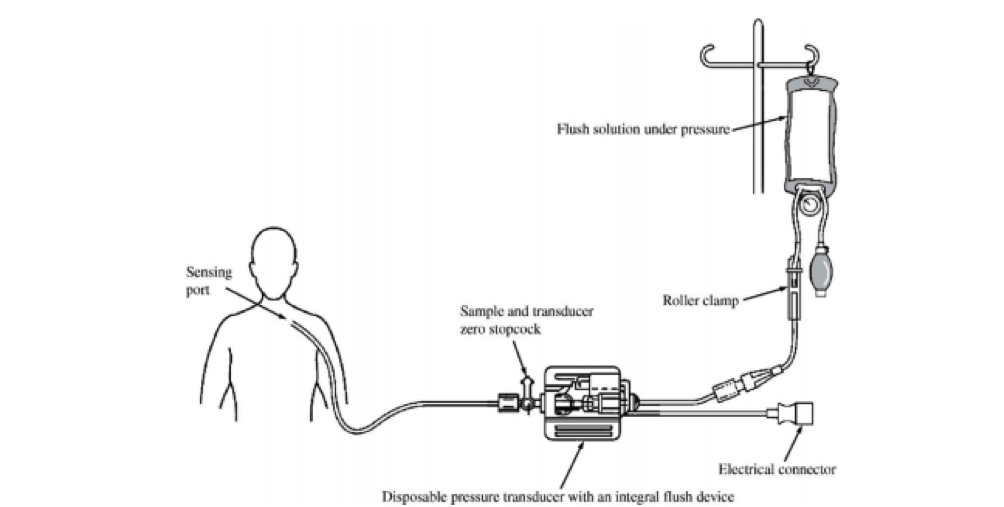
\includegraphics[width=0.8\textwidth]{Figurer/Indledning/Opstilling}
	\label{Opstilling}
	\caption{Tilslutningen af væskefyldt kateter}
\end{figure}
Da det er vigtigt med kontinuerte målinger af blodtrykket bliver målingen foretaget invasivt. På billedet ses det hvordan blodtryksmålesystemet er tilsluttet patientens arterier via et væskefyldt kateter.\\
Projektets resultat vil kunne hjælpe sundhedsfaglig personale med at bevarer overblikket over deres patients fysiske tilstand under en operation. Da det både kan være en planlagt eller akut situation på operationsstuen er det vigtigt, at systemet virker optimalt og udøver den bedste hjælp til personalet.\\
\\  
I dette projekt der skal arbejdes på at udarbejdet et system, der kan tilsluttes det væskefyldte kateter og som kan vise en blodtryks kurve, samt blodtryks værdier på en computerskærm. \\
Systemet skal bestå af to elementer:
\begin{enumerate}
	\item Det ene element består af et elektronisk kredsløb, der forstærker signalet fra transduceren og filtrerer signalet med et indbygget analogt filter.
	\item Det andet element er et program, der afbilder blodtrykket grafisk som funktion af tiden. Programmet skal lige ledes vise blodtryksværdier, samt puls og kunne udløse en alarm hvis grænseværdier for blodtrykket overskrides. 
\end{enumerate}



  

\chapter{Projektformulering}




\textbf{Ansvarsområde} \\
\textbf{Initialer: } \\
Jeppe Tinghøj Honeré - JTH \\
Mads Fryland Jørgensen- MFJ \\
Tine Skov Nielsen- TSN \\
Freja Ramsing Munk - FRM \\
Nicoline Hjort Larsen - NHL \\
Sara-Sofie Staub Kirkeby - SSK \\[2ex]


\begin{longtabu} to \linewidth{@{}  l X[j]@{}}
    Afsnit &    Ansvarlig\\[-1ex]
    \midrule
     
    
    

\end{longtabu}

I dette projekt var problemstilling at lave en invasiv blodtrykmåler til en valgfri institution. Der er i den forbindelse blevet arbejdet med blodtryks-måling, udvikling af hardware til blodtryksmåleren samt udarbejdelse af et program til analyse af blodtryks-målingen.\\ 
\\
Motivationen for projektet bygger på, at der i klinisk praksis ofte er behov for kontinuert at kunne monitorerer en patients blodtryk. Dette er især vigtigt på en operationsstue, hvor blodtrykket er en vigtig parameter til monitorering af deres helbredstilstand, hvilket derfor ligger til grund for udarbejdelsen af dette projekt.\\
\begin{figure}[H]
	\centering
	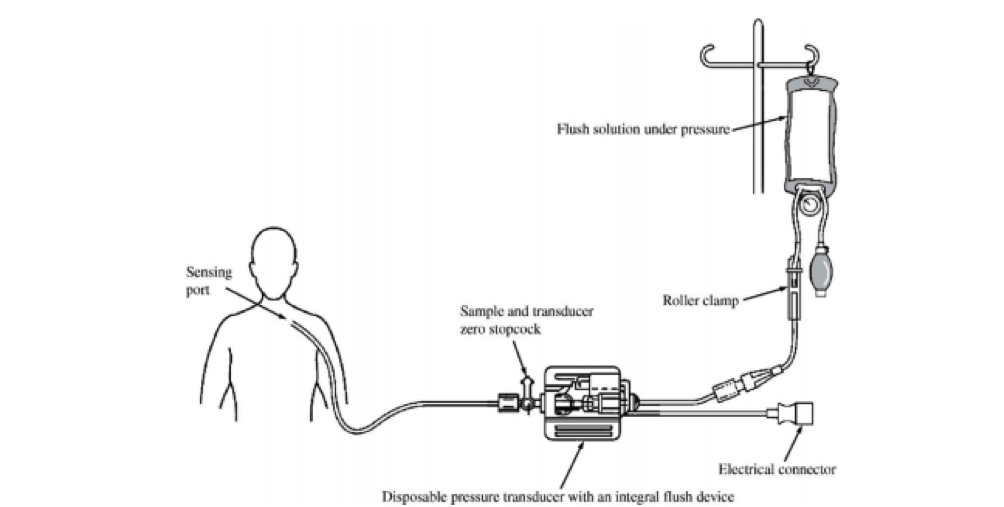
\includegraphics[width=0.8\textwidth]{Figurer/Indledning/Opstilling}
	\label{Opstilling}
	\caption{Tilslutningen af væskefyldt kateter}
\end{figure}
Da det er vigtigt med kontinuerte målinger af blodtrykket bliver målingen foretaget invasivt. På billedet ses det hvordan blodtryksmålesystemet er tilsluttet patientens arterier via et væskefyldt kateter.\\
Projektets resultat vil kunne hjælpe sundhedsfaglig personale med at bevarer overblikket over deres patients fysiske tilstand under en operation. Da det både kan være en planlagt eller akut situation på operationsstuen er det vigtigt, at systemet virker optimalt og udøver den bedste hjælp til personalet.\\
\\  
I dette projekt der skal arbejdes på at udarbejdet et system, der kan tilsluttes det væskefyldte kateter og som kan vise en blodtryks kurve, samt blodtryks værdier på en computerskærm. \\
Systemet skal bestå af to elementer:
\begin{enumerate}
	\item Det ene element består af et elektronisk kredsløb, der forstærker signalet fra transduceren og filtrerer signalet med et indbygget analogt filter.
	\item Det andet element er et program, der afbilder blodtrykket grafisk som funktion af tiden. Programmet skal lige ledes vise blodtryksværdier, samt puls og kunne udløse en alarm hvis grænseværdier for blodtrykket overskrides. 
\end{enumerate}
\textbf{Afgrænsning}\\ \\
Fra IHA’s side er der på forhånd defineret nogle krav til projektets indhold, hvilket indebærer:\\ \\
Software 
\begin{itemize}
	\item Programmet skal programmeres i C\#
	\item Programmet skal kunne kalibrerer blodtrykssignalet og foretage en nulpunktsjustering
	\item Programmet skal kunne vise blodtrykssignalet kontinuert
	\item Programmet skal kunne lagre de måte data i enten en tekstfil eller en database
	\item Programmet skal kunne filtrerer blodtrykket i selve programmet via et digitalt filter, dette skal kunne slås til og fra
\end{itemize}

Hardware
\begin{itemize}
	\item Der skal designes et aktivt 2. ordens lavpasfilter af typen Sallen-Key med unity gain
	\item Filteret skal designes som et Butterworth filter med cut off frekvens på 50 Hz. C2 skal vælges til 680 nF og R1 = R2. Operationsforstærkeren skal være af typen OP27
\end{itemize}
\chapter{Baggrund}
\section{Hjertet \& Kredsløb}
Hjertet, \textit{cor}, er en hul muskel, der har til opgave at pumpe blodet rundt til hele kroppen. Hjertet består af i alt fire kamre, som det kan ses på figur 3.1 nedenfor. To forkamre, atrier, og to hjertekamre, ventrikler. Atrierne fungere primært som reservoir for blod, mens ventriklerne fungerer som den effektive pumpe.\\

\begin{figure}[htb]
	\centering
	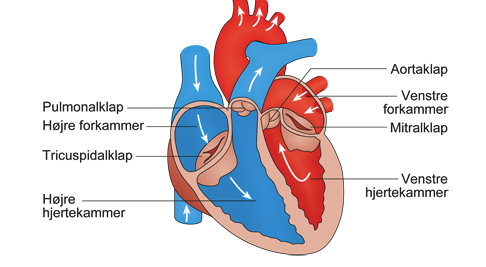
\includegraphics[width=1\textwidth]{Figurer/Fysio/Hjertet}
	\caption{Hjerte med forklarende pile \protect\footnotemark} 
\end{figure}
\footnotetext{http://www.hjertelunge.dk/hjertesygdomme/hjerte\_og\_kredsloeb/hjertet/}

Hjertekamrene og forkamrene er adskilt fra hinanden af anulus fibrosus, som er en plade af bindevæv. Anulus fibrosus består af fire bindevævsringe, der er forbundet med hinanden. To af disse udgør åbningerne mellem atrierne og ventriklerne. De to sidste danner åbningerne mellem højre hjertekammer og lungepulsåren og venstre ventrikel og hovedpulsåren. Ved alle bindevævsringene er der klapper, der fungere som ventiler.\\ 
AV-klapperne sidder mellem atrierne og ventriklerne. Klappen mellem højre atrium og ventrikel kaldes tricuspidalklap, mens klappen mellem venstre atrium og ventrikel kaldes mitralklap, se figur 3.1. Aortaklappen er placeret ved afgangen af hovedpulsåren og pulmonalklappen ved afgangen af lungepulsåren. Klapperne fungere således, at blodet kun kan løbe én vej gennem dem. Åbningen samt lukningen af disse er en passiv proces, som bestemmes af forskelle i væsketrykket på de to sider af klapperne.\\ 

\begin{figure}[htb]
	\centering
	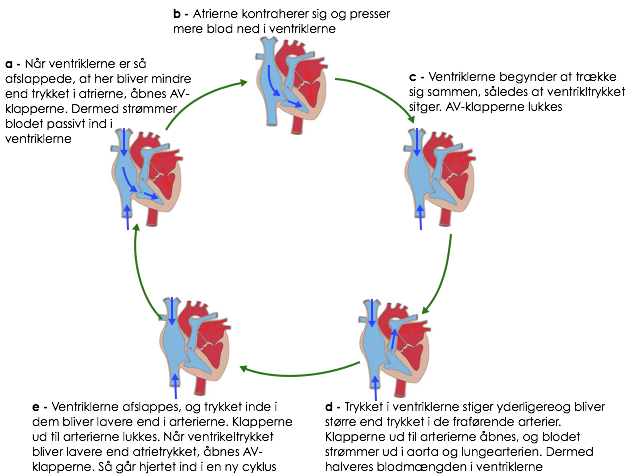
\includegraphics[width=1\textwidth]{Figurer/Fysio/Cyklus}
	\caption{De forskellige faser i hjertets cyklus \protect\footnotemark}
\end{figure}
\footnotetext{Billede fra "Menneskets anatomi og fysiologi" s. 273 figur 9.6}

Hjertets cyklus, som er illustreret ved figur 3.2, inddeles i to hovedfaser. Den første kaldes diastolen. I diastolen er ventriklerne afslappede og fyldes med blod. Det vil sige, at trykket i ventriklerne bliver lavere end trykket i atrierne, således at AV-klapperne åbnes, og blodet begynder at strømme ind i ventriklerne. Under hele diastolen er aortaklappen lukket. Den anden fase kaldes systolen. I systolen kontraherer ventriklerne sig. Trykket i ventriklerne overstiger trykket i atrierne således, at AV-klapperne lukkes, så tilbagestrømning af blod til atrierne forhindres. Når ventriklerne har kontraheret sig så meget, at trykket i ventriklerne overstiger trykket i hovedpulsåren samt i lungepulsåren, åbnes aortaklappen og pulmonalklappen, og blodet strømmer ud i hovedpulsåren og lungepulsåren. Ventriklernes tryk falder igen til under atriernes tryk, hvilket påvirker, at AV-klapperne åbnes igen og hjertets cyklus starter forfra.\\
\section{Blodtryk}
\section{Hypertension}
\section{Hypotension}
\section{Hæmodynamik}


\chapter{Systembeskrivelse}
Systemet, der er blevet udviklet er en blodtryksmåler. Blodtryksmåleren er tiltænkt at fungere som en invasiv blodtryksmåler på operationsstuer, der skal monitorerer patienters blodtryks under operationer.\\
\\ \textbf{Indæst opstilling}
\\
For at kunne lave et sådan system er der blevet udviklet en hardware del og en software del. 
Hardware delen som er bestående af en forstærker og et filter. Forstærkeren forstærker signalerne, der kommer fra en transducer, hvorefter et analogt lavpas filter filtrerer signalet. Transduceren ??? \\ [1ex]

Software delen bestående af en brugergrænseflade samt program med tilhørende database. Brugergrænsefladen viser et digitalt signal via programmet samt giver mulighed for forskellige funktioner og oplysninger. Yderligere består programmet af en mulighed for en digital filtrering af blodtrykssignalet samt algortimer til detektering af systole, diastole og puls. Systemet kan desuden lagre data fra signalet i en privat database.    

Projektets endelig produkt er en prototype af et blodtryksmålings system som kan benyttes til invasiv blodtryksmåling. 



\chapter{Krav}

\chapter{Projektbeskrivelse}

\section{Projektgennemførelse}\label{Projektgennemfoerlse}
Projektet startede med, at der blev lavet en tidsplan, som var mulig at ændre undervejs, dog med faste deadlines, som skulle overholdes. De forskellige deadlines lagde op til, at der kunne arbejdes efter udviklingsmodeller, som er beskrevet nærmere i metodeafsnittet \ref{Metode}.\\ \\
Tidsplanen blev sidenhen ført mere detaljeret ind i projektstryringsværktøjet Scrum. Scrum blev benyttet til at holde overblikket over manglende opgaver, igangværende opgaver og afsluttede opgaver. \\
Gruppens seks medlemmer blev fra start delt op i to undergrupper, én med hovedfokus på hardware udvikling, og én med hovedfokus på software udvikling. Dog blev de basic delene til projektet, som kravspecifikation og case udvalgt samlet. Scrum er her også et godt værktøj til at bevare overblikket over de to gruppers individuelle opgaver.\\ \\
Fra start blev der aftalt et ugentlig møde, med vejleder og de to grupper som medvirkende parter. På denne måde blev alle parter holdt opdateres på udviklingsprocessen, især grupperne imellem, men også vejleder. Sidst i forløbet, under test af diverse dele af systemet, blev grupperne samlet og testene blev udarbejdet i fællesskab.\\ \\
Projektet er gennemført ved udarbejdelse af en samarbejdsaftale, herunder udvælgelse af en projektleder, som i tilfælde af uoverensstemmelse havde den afgørende stemme. 

\section{Metode} \label{Metode}
\subsection{Ase-modellen}
Den primære udviklingsmodel, der er benyttet i dette projekt, er ASE modellen. ASE modellen er en udviklingsmodel, der tager udgangspunkt i use cases. 
\begin{figure}[H]
	\centering
	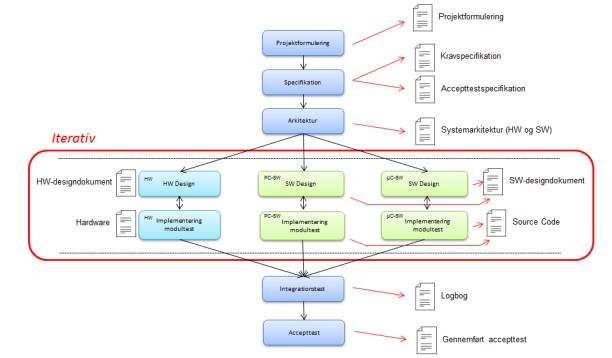
\includegraphics[width=1\textwidth]{Figurer/Metode/ASEmodellen}
	\caption{Projektmodel illustreret med de faser som projektet gennemløber\protect\footnotemark}
	\label{ASEmodel}
\end{figure}
\footnotetext{Fra \textit{"Vejledning til udviklingsprocessen for projekt 2"}}


Modellen er opbygget sådan, at udviklerne benytter vandfaldsmodellen (se afsnit \ref{Vandfald}) til at fastlægge en opgaveformulering, kravspecifikation og systemarkitektur, for derefter at designe og implementere de enkelte moduler i iterationer. \\ Ud fra projektformuleringen specificeres kravspecifikationen som en række use cases. Use cases er et værktøj, der beskriver diverse aktørers interaktion med systemet. Ved at definere kravspecifikationen ud fra use cases, opnås et overblik over hvilke krav, der stilles til systemets endelige funktionalitet.\\ \\ Ud fra kravspecifikationen kan systemets accepttest udarbejdes. Efter kravspecifikationen er fastlagt, udarbejdes systemarkitekturen.\\ I systemarkitekturen uddeles systemets funktionalitet i moduler og deres grænseflader til resten af systemet bestemmes. Ud fra systemarkitekturen designes systemet ved at nedbryde det efter funktionalitet, som kan bindes til både hardware og software.
\subsection{Vandfald}\label{Vandfald}
Denne metode bygger pa at gøre en hel fase af arbejdet færdigt før den næste startes. Grafisk ser det ud som på figur \ref{Vandfaldsmodel}: \\

\begin{figure}[H]
	\centering
	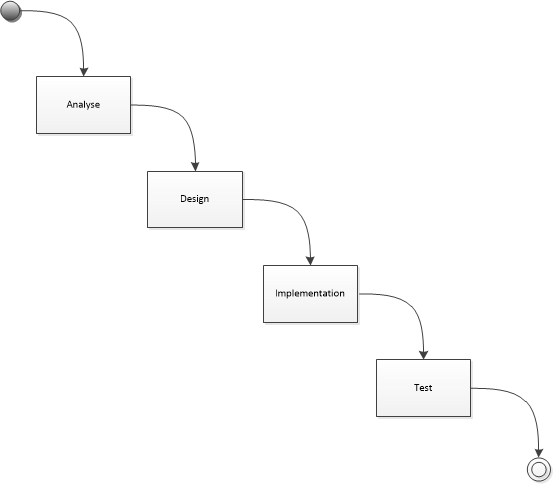
\includegraphics[width=0.8\textwidth]{Figurer/Metode/Vandfald}
	\caption{Vandfaldsmodel}
	\label{Vandfaldsmodel}
\end{figure}
Projektet starter med en analyse, og så videre med de andre faser - design, implementering og test. Det er altså hele systemet, der arbejdes igennem i hver fase, og vandfaldet symboliserer, at der kun arbejdes i en retning, altså man kan ikke gå imod strømmen. Metoden benyttes, når opgaven er veldefineret og velkendt. \\
Projekt forløbet skal have en kort varighed, dvs. mindre end ca. 4 måneder, under velkendte forhold med hensyn til udviklings- og testmiljø, udviklingsmetodik, platforme etc. \cite{Projektledelse}

\subsection{V-model}
V-modellen er en model, hvor testen planlægges parallelt med udviklingen. Accepttesten planlægges detaljeret efter kravnalysen, altså kravspecifikationen, systemtest planlægges detaljeret efter system design, og integrationstesten planlægges detaljeret efter arkitektur design fasen. Unit/modul testen ligger dog uændret i forhold til den traditionelle strategi.
\begin{figure}[H]
	\centering
	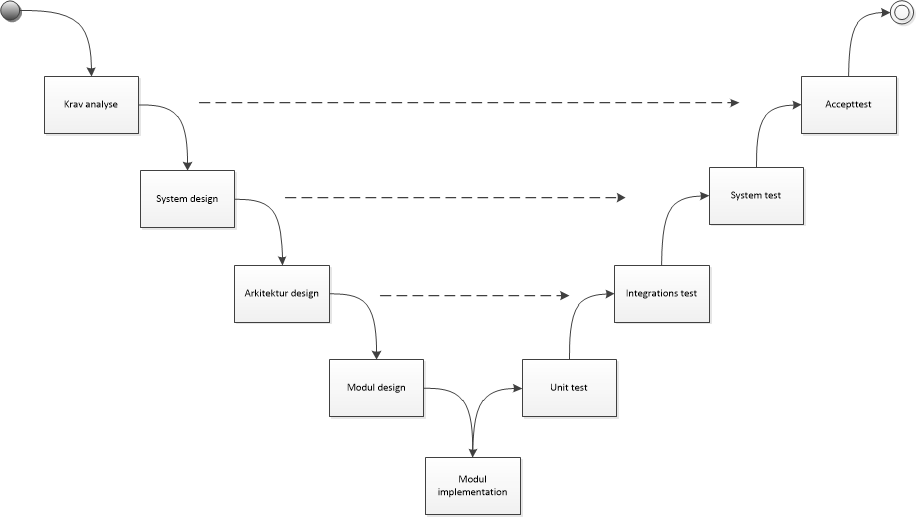
\includegraphics[width=1\textwidth]{Figurer/Metode/Vmodel}
	\caption{V-model}
	\label{Vmodel}
\end{figure}
Testens praktiske udførelse er altså uændret i forhold til Ase-modellen og Vandfaldsmodellen, dvs. den ligger sidst i forløbet. Det betyder at testfaserne planlægges modsat den rækkefølge, de udføres i. Den største forskel for testerne er, at planlægningen baseres på de tidlige modeller af systemet, ikke på det færdige system. \\
 V-modellen udvides desuden med reviews og deadlines (se afsnit \ref{Projektgennemfoerlse}).

\section{Specifikation og analyse}



\section{Arkitektur}
I det følgende afsnit beskrives arkitekturen for systemet. Systemarkitekturen fungerer her som udviklingsramme for videre design og implementering. Her bliver systemets funktionalitet 
nedbrudt til overordnede moduler. \\
   Arkitekturen for projektet er foretaget i to dele - en hardware arkitektur og en software arkitektur. Arkitekturen beskriver opbygningen af systemet i form af diagrammer.  
   \subsection{software arkitektur}
   I software designet er der udarbejdet en domæne model, der giver et overblik over hele systemet.
 \begin{figure}[H]
	\centering
	\includegraphics[width=1\textwidth]{Figurer/ISE/Domaenemodel}
	\caption{Domænemodel}
	\label{domaenemodel}
\end{figure}
   I domæne-modellen er relationerne mellem aktørerne og systemets dele beskrevet med pile og vejledende tekster - dette skulle gerne give et større overblik over systemets funktionalitet. \\ 
   En domænemodel beskriver dog ikke, hvilken rækkefølge de forskellige handlinger sker i, og derfor er der udarbejdet sekvensdiagrammer for hver use case for systemet, som skal beskrive dette.\\
   Her ses sekvensdiaframmet for use casen "Mål blodtryk"
    \begin{figure}[H]
	\centering
	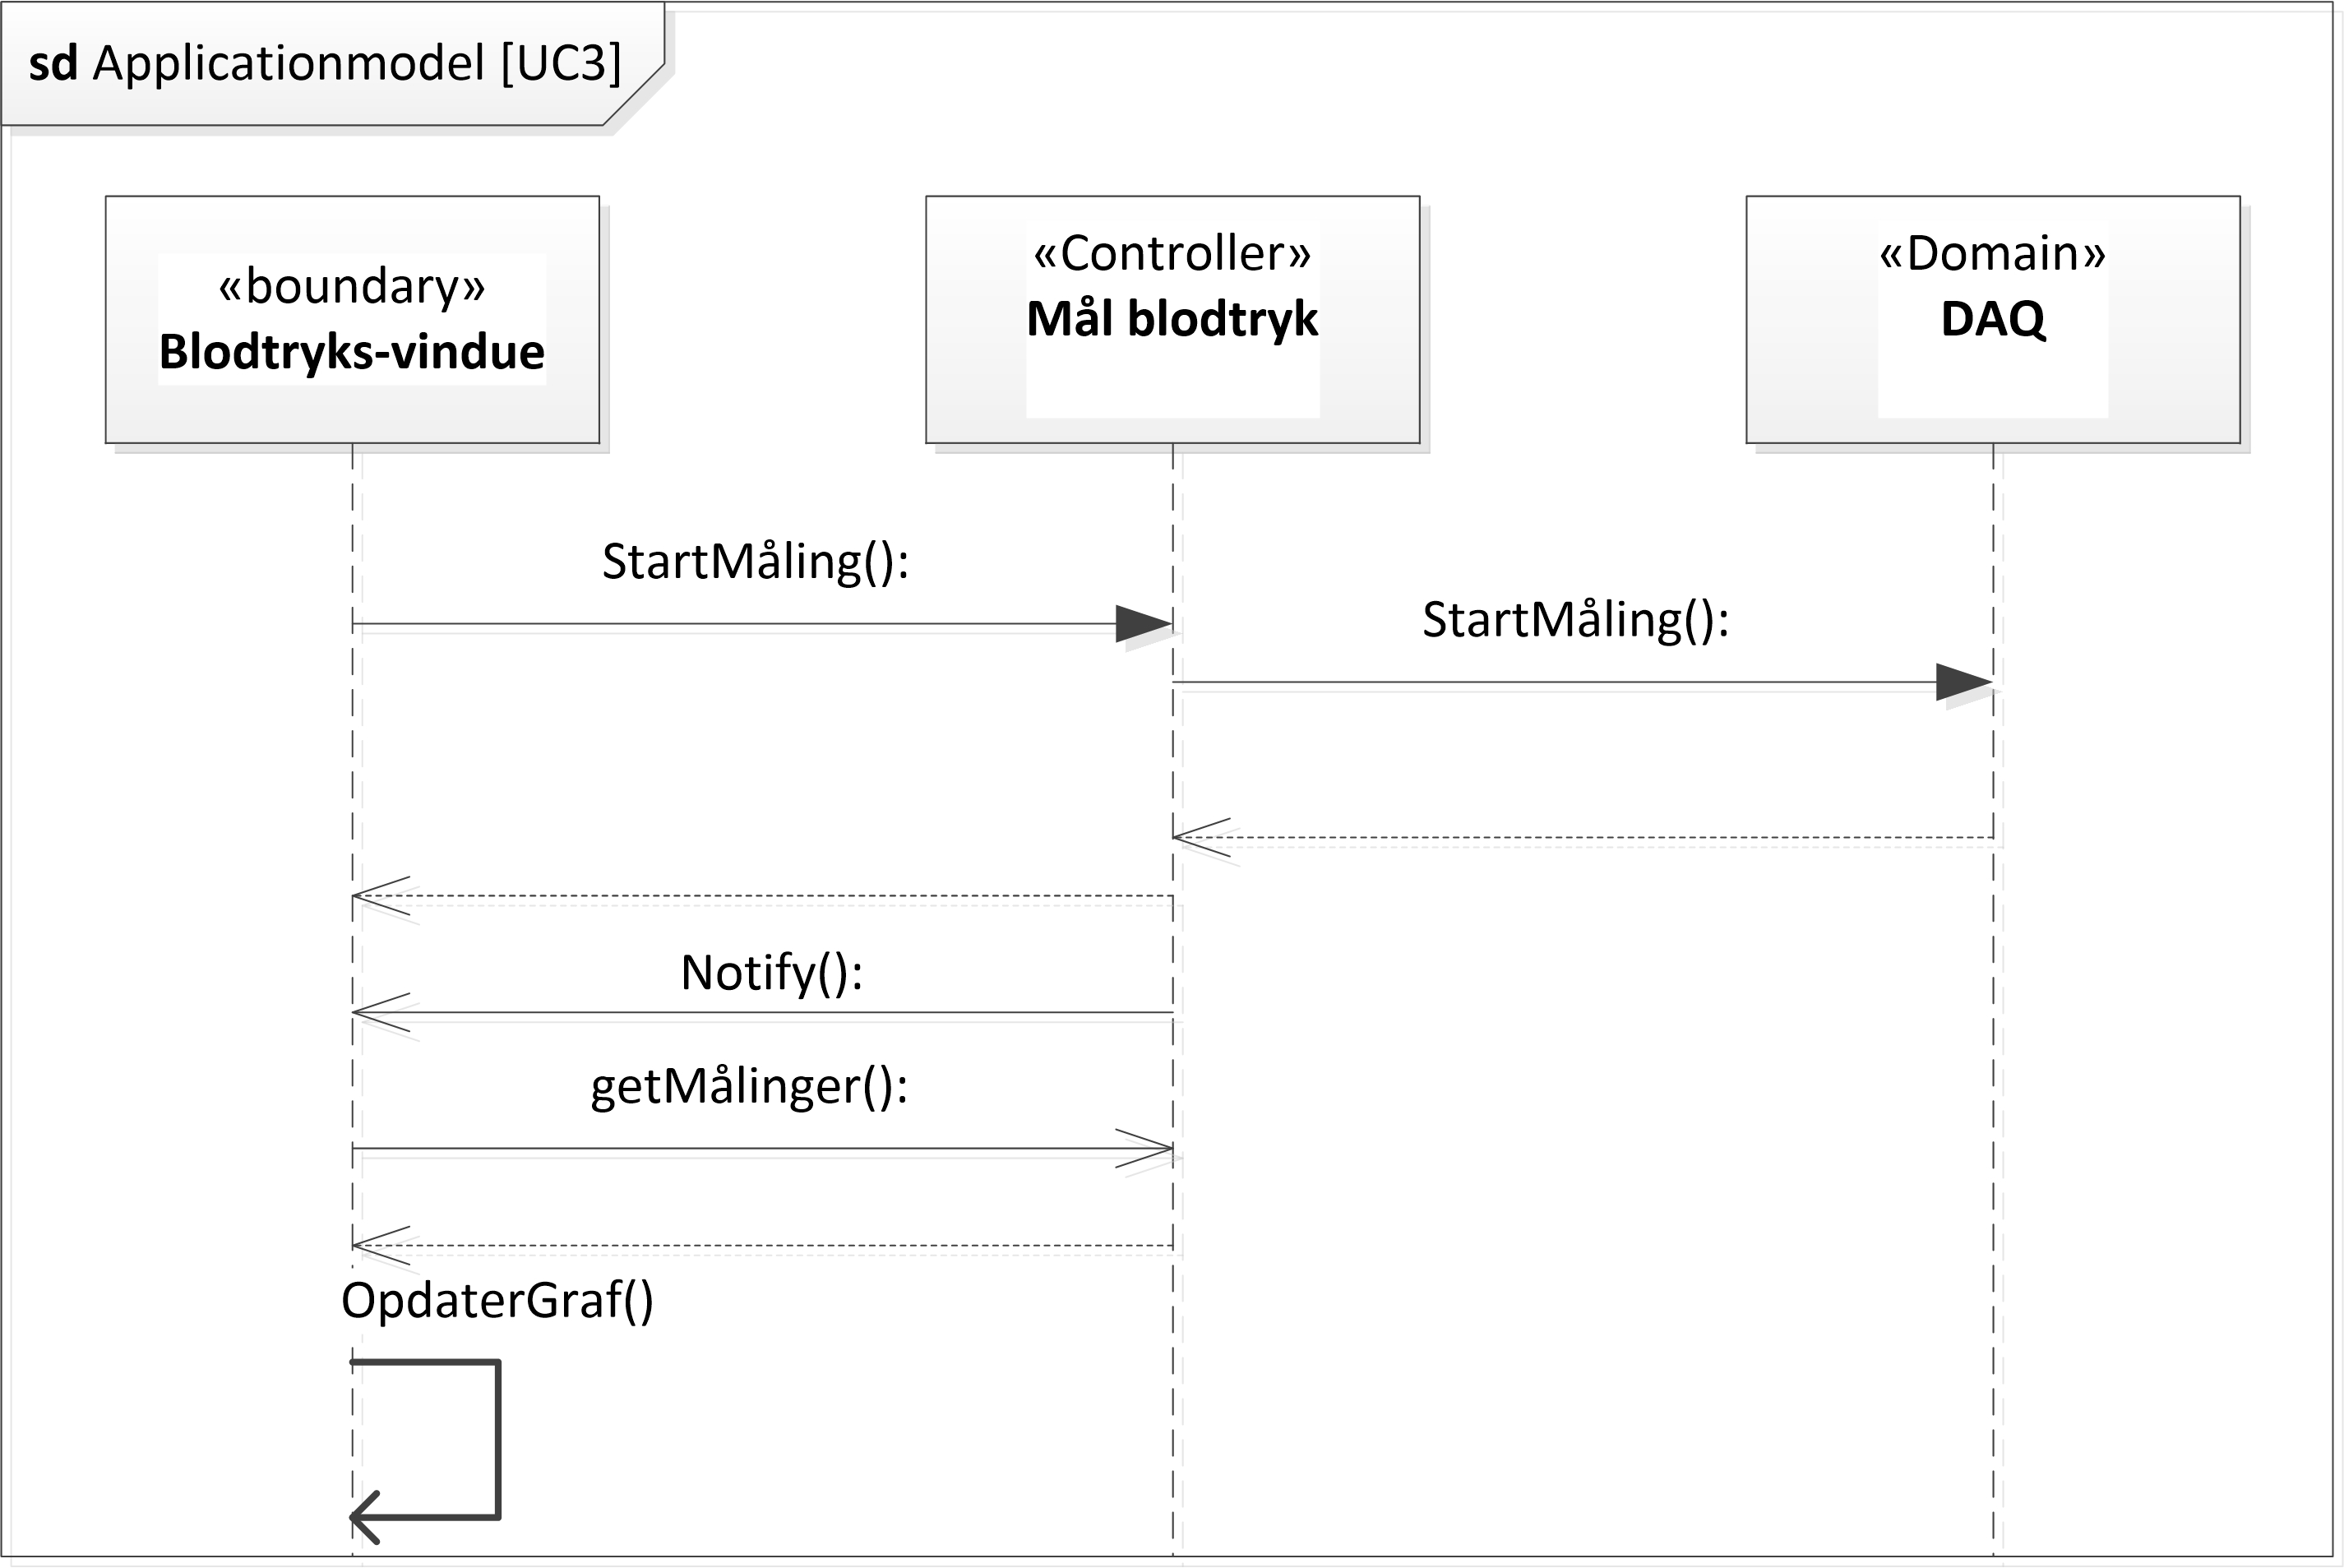
\includegraphics[width=1\textwidth]{Figurer/ISE/sdAppModelUC3}
	\caption{Sekvensdiagram UC3}
	\label{sekvensdiagram}
\end{figure}
Her ses det hvordan brugeren interagerer med brugergrænsefladen ved at starte blodtryksmålingen. Herefter bliver metoden til at starte blodtryksmålingen kaldt ned gennem logik- og datalag hvor efter målingen vises i en graf på brugergrænsefladen. Grafen bliver hele tiden opdateret med nye målinger.\\
Ud fra dette kan det ses hvordan brugerens interaktion med brugergrænsefladen sætter gang i metoder i software programmet. Skevensdiagrammet giver altså et overblik over hvordan softwaren er bygget op.\\
Sekvensdiagrammerne for de øvrige use cases kan ses i dokumentationen afsnit ....
  
 \subsection{SysML}
 I beskrivelsen af systemarkitekturen og det detaljerede design for det færdige produkt, er der 
anvendt SysML. SysML kommer originalt fra UML, men UML er hovedsagligt centreret omkring udvikling af software systemer. Da det udviklede system både består af hardware og software, er der valgt SysML til arkitekturen.\\
Valget af SysML grunder også i, at det giver en god formidling af systemet - dette giver udviklerne et større overblik. Samtidig er det også let for en udenforstående at sætte sig ind i systemets kunnen.\\

I dette projekt er der benyttet struktur- og adfærdsdiagrammer til at specificere og 
dokumentere systemet. Som strukturdiagram er der anvendt et blok definitions diagram (bdd) samt interne blok definitions diagramm (ibd).\\
Der er anvendt adfærdsdiagrammer i form af sekvensdiagrammer i dette projekt. Disse 
diagrammer er velegnet til sekventielt at beskrive den logiske funktionalitet i systemet.
Softwaren er opbygget ud fra sekvensdiagrammer beskrevet i arkitektur afsnittet. 



\subsection{Design}


\subsection{Implementering}
Herefter blev de to blokke bygget op. Gruppen valgte at bygge forstærkeren og filteret på hver sit fumlebræt, dels på grund af pladsmangel og dels på grund af større sammenhæng mellem arkitekturen, og det endelige produkt.\\

    \begin{figure}[H]
	\centering
	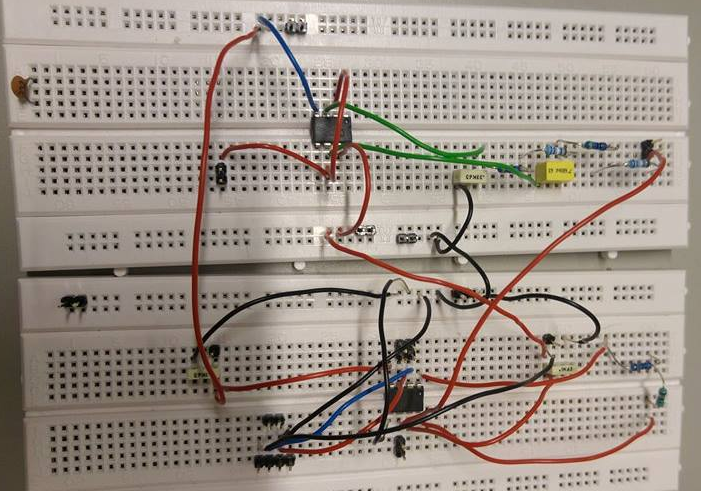
\includegraphics[width=1\textwidth]{Figurer/Hardware/samletopstilling}
	\caption{Opbygning af forstærker og filter}
	\label{samletopbygning}
\end{figure}

Grundet mangel på præcise modstande, bedømte gruppen at det var bedst at bygge modstandende i forholdsvist filteret og forstærkeren, op i to, så gruppen kunne komme så tæt på den ønskede modstandsværdi som muligt. \\

\subsubsection{Implementering af forstærkeren}
Den samlede stykliste for forstærkeren blev vist som på tabel \ref{forsttabel}.

\begin{center}
\begin{tabular}{|c|c|c|}
\hline 
Komponent & Antal & Type \\ 
\hline 
Modstand & 1 & 120\\
\hline
Modstand & 1 & 4,8\\
\hline
Kondensator & 2 & 100 nF\\
\hline
Instrumentationsforstærker & 1 & INA114 \\ 
\hline
\end{tabular} 
\label{forsttabel}
\end{center}

For forstærkeren gælder det at den beregnede $R_{gain}$ er 125,31\Ohm som det kan ses ud af komponentlisten består RGain i praksis af to modstande på henholdsvis 4,8Ω og 120Ω som er sat i serie. $R_{gain}$ modstanden er i praksis 124,8\Ohm. I praksis er $R_{gain}$ 0,51\Ohm mindre end den i teorien skulle have været.

\subsubsection{Implementering af filteret}
Den samlede stykliste for filteret blev som vist på tabel \ref{filtertabel}.

\begin{center}
\begin{tabular}{|c|c|c|}
\hline 
Komponent & Antal & Type \\ 
\hline 
Modstand & 2 & 6.2 k \\ 
\hline 
Modstand & 2 & 470\\
\hline
Kondensator & 1 & 680 nF\\
\hline
Kondensator & 1 & 330 nF\\
\hline
Operationsforstærker & 1 & OP27G \\ 
\hline
\end{tabular} 
\label{filtertabel}
\end{center}

Det analoge filter består blandt andet af en 330 nF kondensator, $C_{1}$, som i teorien er beregnet til at skulle have været 333,2 nF. I praksis er kondensatoren $C_{1}$ 3,2 nF mindre end den i teorien er beregnet til at skulle have været. Filteret består desuden af to modstande $R_{1}$ og $R_{2}$ som er identiske. I det realiserede analoge filter består hver modstand af to modstande på henholdsvis 6200\Ohm og 470\Ohm som er sat i serie. Dermed er både $R_{1}$ og $R_{2}$ 6670\Ohm i praksis. I teorien var $R_{1}$ og $R_{2}$ udregnet til at skulle være 6687\Ohm. I praksis er der derfor 17\Ohm mindre end teorien foreskriver.\

Generelt er der valgt at se bort fra de afvigelser, der er for komponentværdierne i praksis sammenlignet med de i teorien beregnet. Det er valgt da afvigelserne er relativt små i forhold til det pågældende komponent. For modstandende er der desuden 1 procents usikkerhed, hvilket betyder man alligevel ikke kan være helt sikker på komponentværdien.\

På baggrund af de i praksis anvendte komponenter er den reelle knækfrekvens for det analoge filter beregnet. Til det formål er formlen anvendt.\

CUTOFFFREKVENS!?

\subsection{Test}


\section{Resultater og diskussion}


\section{Opnåede erfaringer}


\section{Fremtidigt arbejde}

\chapter{Konklusion}
I forgående projekt, er der blevet udviklet en blodtrykssystem prototype, bestående af både software og hardware, som er i stand til, at måle og vise intravenøst blodtryk. \\
\\
Gruppen startede med at fremlægge forholdsvist realistiske krav til prototypen. Disse krav blev dog ændret i løbet af udviklingsfasen, fordi nogen af kravene, ikke passede sammen. Dette gjorde sig især gældende i hardware kravene, som omhandlede forstærkning og forsyningsspænding. Også i software delen, var der dog behov for at sortere enkelte mindre designrelaterede krav fra.  \\
\\
Der er forsøgt fokuseret på, hvordan et sådan system, ville skulle fungere ude i virkeligheden. Dette kan ses på de krav, som gruppen selv har sat, ud over de fastlagte IHA krav. Efter kravene blev modificeret, er det dog lykkedes gruppen at leve op til alle de krav, som der blev sat til projektet. \\
\\

Ideelle tanker kontra realitet??\\
Da accepttesten blev gennemført, var der ingen behov for at skrive nogen fejlrapporter, da alle krav kunne eftervises og testes i programmet. Enkelte tekniske krav var dog nødt til, at blive eftervist i større omfang, i separate test afsnit. De større krav omkring at måle, filtrere og afbillede et blodstryks signal blev opfyldt til fulde. Alle mindre krav er desuden også implementeret med succes. \\
\\
Selve udviklingen af systemet, har været meget præget af, at gruppen har været delt i to. Der har været svag kommunikation imellem de to grupper, men på trods af dette er det lykkedes gruppen at få udviklet to dele, som kunne arbejde sammen. \\
\\
Generelt set, mener gruppen at projektet er gået godt, og at det system, som er blevet udviklet, er klar til at blive udviklet yderligere, skulle det være en mulighed. \\
\\

\begin{thebibliography}{9}
	
	\bibitem{Statistik}
	sundhed.dk,
	\emph{Højt blodtryk}
	URL:\url{https://www.sundhed.dk/sundhedsfaglig/laegehaandbogen/hjerte-kar/symptomer-og-tegn/hoejt-blodtryk/},
	version 02.08.2015
	
	\bibitem{blodtryk}
	Webster, John G., m.fl.,
	\emph{Medical Intrumentering},
	John Wiley \& Sons, INC, ISBN-13 978-0471-67600-3
	 
	 
	\bibitem{Hjertet}
	Hjerteforeningen,
	\emph{Hjertet},
	URL:\url{http://hjertesvigt.dk/hjertesygdomme/hjerte_og_kredsloeb/hjertet/},
	version 11.11.2014
	
	\bibitem{cyklus}
	Sand, Olav, m.fl.
	\emph{Menneskets anatomi og fysiologi},
	s. 273 figur 9.6,
	Gads Forlag,
	2. udgave, 3. oplag,
	2008, ISBN 978-87-12-04298-3. 
	
	\bibitem{haemo}
	Gyldendal, Den Store Danske,
	\emph{blodtryk}
	URL:\url{http://www.denstoredanske.dk/Krop,_psyke_og_sundhed/Sundhedsvidenskab/Fysiologi/blodtryk},
	version 23.10.2009
	
	\bibitem{tryk}
	Johansen, Peter,
	\emph{Hæmodynamik og hjertekarsystemet},
	s. 33,
	5. udgave,
	Note fra KVI undervisning 2015
	
	\bibitem{Hypertension}
	sundhed.dk,
	\emph{Hypertension}
	URL:\url{https://www.sundhed.dk/sundhedsfaglig/laegehaandbogen/hjerte-kar/tilstande-og-sygdomme/oevrige-sygdomme/hypertension/},
	version 04.08.2015
	
	\bibitem{Hypotension}
	sundhed.dk,
	\emph{Shock}
	URL:\url{https://www.sundhed.dk/sundhedsfaglig/laegehaandbogen/akut-og-foerstehjaelp/tilstande-og-sygdomme/hjerte-kar/shock/},
	version 19.08.2015
	
	\bibitem{IHA modellen}
	Ingeniørhøjskolen Aarhus Universitet,
	\emph{Vejledning til dokumentation af semesterprojekter},
	udgave 29.4.2015
	
	
	\bibitem{Projektledelse}
	Poul Staal Vinje,
	\emph{Projektledelse af systemudvikling},
	Nyt Teknisk Forlag,
	ISBN 978-87-571-2457-5.
	
	\bibitem{Overforing}
	OKAWA Electric Design,
	\emph{Sallen-Key Low-pass Filter Design Tool},
	URL:\url{http://sim.okawa-denshi.jp/en/OPseikiLowkeisan.htm}
	Version 2008
	
	
	\bibitem{elbog}
	Thomas, Rosa \& Toussaint,
	\emph{Analysis and Design of Linear Circuits},
	Wiley,
	7. udgave, 
	2012, ISBN  978-11-180-6558-7. 
	
	
\end{thebibliography}


%\cite{Projektledelse} henviser til bibitem Projektledelse og tilføjer [1] det sted man henviser fra


\backmatter


%\bibliography{bibliografi/PRJ3}    % Sætter bibliografien bagerst i dokumentet. Bruger bib-filen PRJ3.

\end{document}